\chapter{Volumes of balls and cubes; Lattice Polytopes}

\scribe{Victor Bravo}

\section{Comparing the volumes of balls and cubes}

Given an $n$-dimensional ball of radius $r$, we have that
$\text{vol}(B^{n}_{r}) = \dfrac{\pi^{\frac{n}{2}}}{\Gamma(\frac{n}{2}
  + 1)}r^{n}$, where $\Gamma$ is the Gamma Function, which is defined
in the following way:

\begin{enumerate}

\item $\Gamma(m + 1) = m !$, for $m \in \mathbb{N}_{0}$.

\item $\Gamma(m + \frac{1}{2}) = \dfrac{(2m)!}{m! 4^{m}}\sqrt{\pi}$.
\end{enumerate}

\begin{example} $\text{vol}(B^{1}_{r}) = \dfrac{\sqrt{\pi}}{\Gamma(1 + \frac{1}{2})}r = \dfrac{1!\sqrt{\pi}4^{1}}{2!\sqrt{\pi}}r = 2r$.
\end{example}
\begin{example} $\text{vol}(B^{2}_{r}) = \dfrac{\pi}{1!}r^{2} = \pi r^{2}$.
\end{example}

Now, we want to know the asymptotic behaviour, i.e., having a cube
with a ball inside, we want to know how evolves the volume of the cube
compared with the volume of the ball. Using the unit cube, in
dimension $1$, we have the same volume for the cube and the ball
because they are the same thing. In dimension $2$ (see figure 1), we
have a square with every edge of length $1$ and then, the ball has
radius $1/2$. In dimension $3$ (see figure 2), we have a cube with
every edge of length $1$ and then, the ball also has radius $1/2$,
etc.

\begin{figure}
\centering
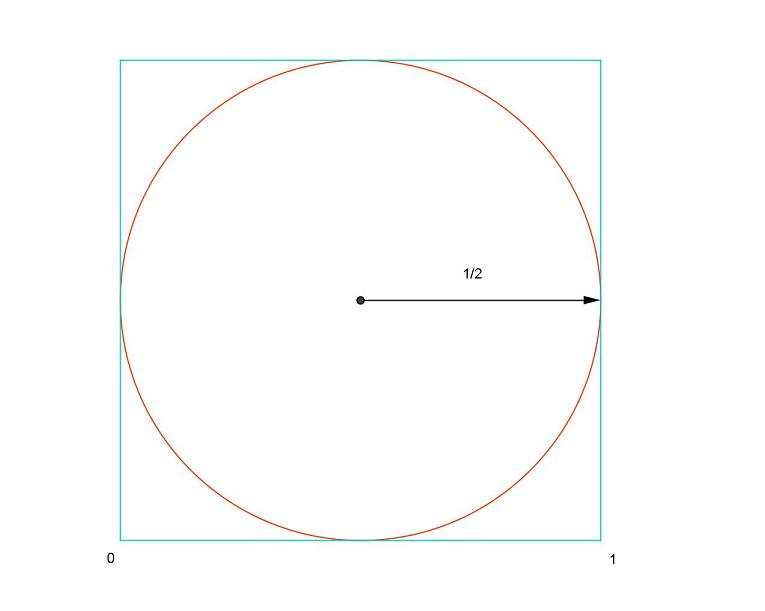
\includegraphics[width=0.5\textwidth]{figure1.jpg}
\caption{Example in dimension $2$.}
\end{figure}

\begin{figure}
\centering
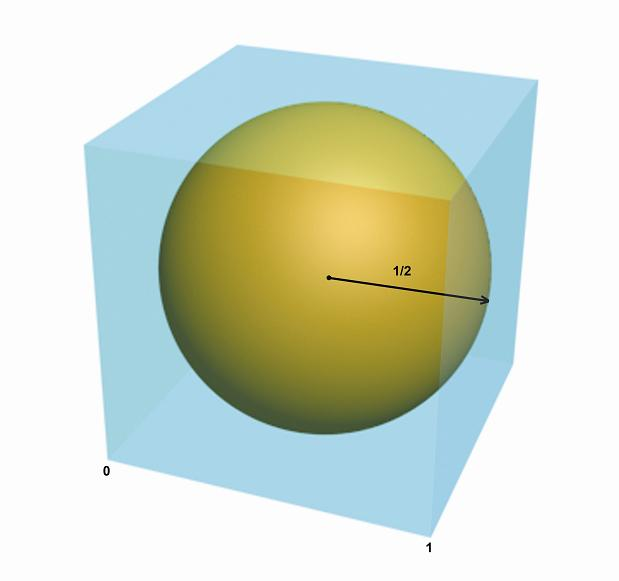
\includegraphics[width=0.5\textwidth]{figure2.jpg}
\caption{Example in dimension $3$.}
\end{figure}

Then, the general case is,
$\dfrac{\text{vol}(B^{n}_{1/2})}{\text{vol}(_{0}^{}\square_{1}^{n})} =
\text{vol}(B_{1/2}^{n}) =$ fraction of unit cube taken up by largest
ball contained inside.

Now, using Stirling's approximation, $\Gamma(x + 1) \approx \sqrt{2
  \pi x}\left(\dfrac{x}{e}\right)^{x}$, $x \in \mathbb{R}_{\geq 0}$,
we have that asymptotically,

$\text{vol}(B_{1/2}^{n})
\stackrel{n \rightarrow \infty}{\longrightarrow}
\dfrac{\pi^{\frac{n}{2}}(\frac{1}{2})^{n}}{\sqrt{2 \pi\frac{n}{2}}(\frac{n/2}{e})^{\frac{n}{2}}} =
\dfrac{\pi ^\frac{n}{2} 2^\frac{n}{2} e^\frac{n}{2}}{\sqrt{\pi n} n^\frac{n}{2} 2^{n}} =
\dfrac{1}{\sqrt{\pi n}}\left( \dfrac{\pi e}{2n} \right)^{\frac{n}{2}} 
\stackrel{n \rightarrow \infty}{\longrightarrow}
0$.

\begin{example} $\dfrac{\text{vol}(B_{1/2}^{100})}{\text{vol}(\square^{100})} \approx 10^{-67}$.
\end{example}

Then, we have bad news for numerical integration (for example in the
case of Monte Carlo integration) when it is used in physics or in
financial mathematics because, by the example above, we will be not
able to count from $1$ to $10^{-67}$. This is too long. So, this works
worst as the dimension increases. In conclusion, we will not use Monte
Carlo Integration to calculate volumes in high dimensions because the
volumes of the balls will be so tiny.

\begin{remark} An example of Monte Carlo Integration in physics
  consists in throw random points into our space and count how many
  points fall inside and how many points fall outside. Then, do the
  fraction which divides the number of points inside and the number of
  points thrown and this fraction approximates the volume (it is used
  at CERN). In the other hand, Monte Carlo Integration is used in
  financial mathematics, for example if we have a portfolio with many
  variables and we have to integrate, one way to integrate by all this
  variables is using Monte Carlo Integration.
\end{remark}


\section{Lattices and lattice polytopes}

Now, we will talk about lattice packings of spheres. A lattice has two
different meanings in mathematics: a partially ordered set or a
group. We are gonna talk about the group.

The most important lattice is $\mathbb{Z}^{d}$, and it's called the
integer lattice. This is an abelian group with the sum: $x, y \in
\mathbb{Z}^{d} \Rightarrow - x \in \mathbb{Z}^{d}, x + y \in
\mathbb{Z}^{d}$, and the sum is commutative.

Now, if we have $v_{1}, \ldots, v_{n} \in \mathbb{Z}^{d}$, and we have
a look to $P = \text{conv}\lbrace v_{1}, \ldots, v_{n} \rbrace
\subseteq \mathbb{R}^{d}$, we define a lattice polytope as the convex
hull of a finite set of points with integer coordinates.

\begin{figure}
\centering
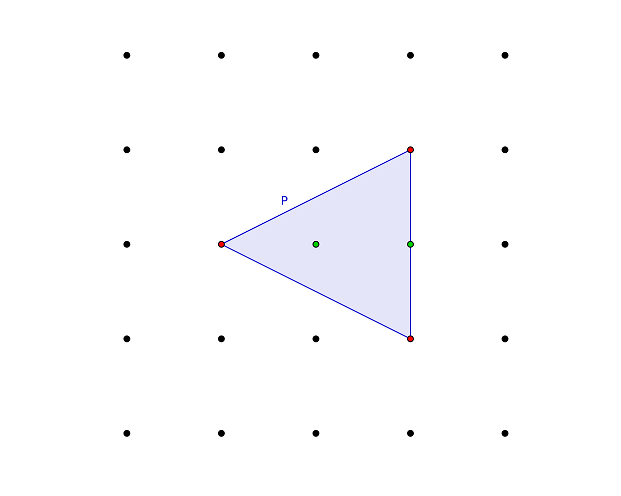
\includegraphics[width=0.5\textwidth]{figure3.png}
\caption{A lattice triangle.}
\end{figure}

Now, we can do the next question: When two lattice triangles "the
same"? The first observation is that we have to answer is: When two
polytopes are "the same"? In Figure 4, we can say that the two lattice
triangles are "the same" because they share all properties respect to
the lattice.

\begin{figure}
\centering
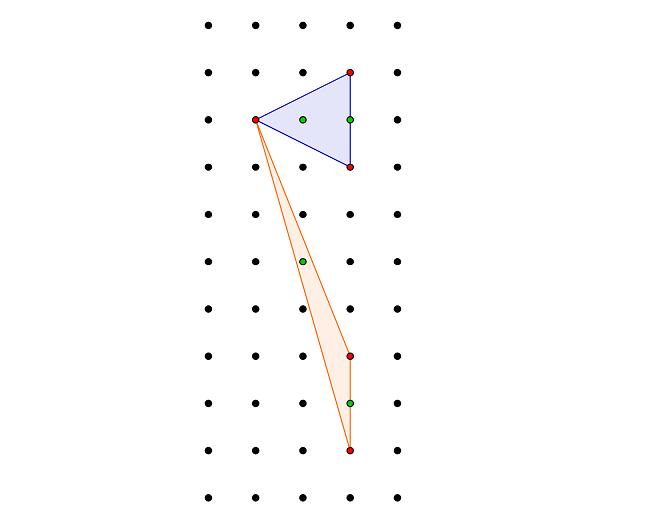
\includegraphics[width=0.5\textwidth]{figure4.png}
\caption{Two lattice triangles.}
\end{figure}

Now, forgetting lattices, the answer to the question for polytopes in
general is: Klein's Erlangen Program. In this program, Klein
identifies the geometry with the groups of automorphisms, i.e., what
Klein makes is to say what the geometry is, by seeing which group of
automorphisms leaves certain object invariant.

Some groups that we must have in mind are $O(n, \mathbb{R}) = \lbrace
A \in \mathbb{R}^{n \times n} : A^{-1} = A^{T} \rbrace$ and $SO(n,
\mathbb{R}) = O(n, \mathbb{R}) \cap \lbrace A \in \mathbb{R}^{n \times
  n} : \det A = 1 \rbrace$. In the other hand, we can also have in
mind the set of translations in $\mathbb{R}^{n \times n}$, $T(n,
\mathbb{R}^{n \times n})$, which satisfies $SO(n, \mathbb{R}^{n \times
  n}) \rtimes T(n, \mathbb{R})$, where $\rtimes$ is the semi-direct
product, which means: two subsets, $P, Q \subseteq \mathbb{R}^{n}$,
are ''the same'' if $\exists A \in O(n)$ and $\exists t \in
\mathbb{R}^{n} : Q = A \cdot P + t$, i.e., I can obtain $Q$ from $P$
through a rotation $A$ and a translation $t$ (i.e., $P$ and $Q$ are
congruent), and this is what we know as Euclidean Geometry.

Now, remembering lattices, we have to change the euclidean geometry by
lattice geometry, i.e., we want bijective homomorphisms that preserves
the lattices. So, we want to determine $\text{Aut}(\mathbb{Z}^{d}) =
\lbrace \text{affine transformations that leave } \mathbb{Z}^{d}
\text{ invariant} \rbrace$, and this is to find conditions on $A \in
\mathbb{R}^{n \times n}$ and $t \in \mathbb{R}^{n}$ such that $Ax + t
\in \mathbb{Z}^{d}$, $\forall x \in \mathbb{Z}^{d}$.
These conditions are:

\begin{itemize}
\item $x = 0$, want $A \cdot 0 + t \in \mathbb{Z}^{d}
  \Longleftrightarrow t \in \mathbb{Z}^{d}$.

\item $x = e_{i}$, with $e_{i}$ a generating vector of our lattice,
  want $A \cdot e_{i} \in \mathbb{Z}^{d} \Longleftrightarrow$ every
  column of $A \in \mathbb{Z}^{d} \Longleftrightarrow A \in
  \mathbb{Z}^{d \times d}$.
\end{itemize}

Now, for $A$ to be an automorphism, it must be invertible, and
$A^{-1}$ must belong to $\mathbb{Z}^{d \times d}$.

\begin{example} Suppose that $d = 2$. We have
  $\left( \begin{smallmatrix} a & b \\ c & d \end{smallmatrix} \right)
  \in \mathbb{Z}^{2 \times 2}$. Then, $A^{-1} = \frac{1}{ad - bc}
  \left( \begin{smallmatrix} d & -b \\ -c & a \end{smallmatrix} \right) =
  \frac{1}{\det A}\left[ (c_{ij}) \right]$, where $(c_{ij})$
  represents the cofactors of $A$. And $A^{-1} \in \mathbb{Z}^{2
    \times 2}$ because $ad - bc$ never divides the entries of
  $\left( \begin{smallmatrix} d & - b \\ - c & a \end{smallmatrix}
  \right)$. (This has to be proved.)
\end{example}

Then, $\text{Aut}(\mathbb{Z}^{d}) = \left\lbrace A \in \mathbb{Z}^{d
    \times d} : \det A = \pm 1 \right\rbrace \rtimes \mathbb{Z}$.

Observe that the set of orientation-preserving linear (not affine)
automorphisms of $\mathbb{Z}^{d}$ is $\Sl_d(\ZZ) = \big\{ A \in
\mathbb{Z}^{d \times d} : \det A = 1 \}$, the special linear group
with integer coefficients. On the other hand, $\left\lbrace A \in
  \mathbb{Z}^{d \times d} : \det A = -1 \right\rbrace$ is not a group.

  Then, what lattice geometry means is that geometry with group
  automorphisms: $Sl_{d}(\mathbb{Z}) \rtimes \mathbb{Z}^{d}$, and this
  is mapping $x \longmapsto Ax + t$, with $t \in \mathbb{Z}^{d}$, $A
  \in \mathbb{Z}^{d \times d}$, and $\det A = \pm 1$. Then, any two
  lattice polytopes in correspondence by any of this automorphisms
  will be the same polytope.

  Now, observe that in Figure 4, using that the image of the vectors
  are the same than the columns of the matrix $A$, we have that $A =
  \left[ \begin{smallmatrix} 1 & 0 \\ -2 & 1 \end{smallmatrix}
  \right]$, with $A \cdot e_{1} = \left( \begin{smallmatrix} 1 \\ -
      2 \end{smallmatrix}
  \right)$ and $A \cdot e_{2} = \left( \begin{smallmatrix} 0 \\
      1 \end{smallmatrix} \right)$.  Also, observe that the following
  transforms (called \emph{shears}) are typical lattice transforms in
  $\mathbb{Z}^{2}$: $\left[ \begin{smallmatrix} 1 & 0 \\ * &
      1 \end{smallmatrix} \right]$ and $\left[ \begin{smallmatrix} 1 &
      * \\ 0 & 1 \end{smallmatrix} \right]$. This can be used in
  exercise 3 of list 1.

After seen this, we are going to see some definitions:

Let $P \subseteq \mathbb{R}^{d}$ be a polytope ($\sim$ convex hull of
finitely many points). A linear inequality of the form $ax \leq b$
with $a \in (\mathbb{R}^{d})^{*}$, $x \in \mathbb{R}^{d}$, $b \in
\mathbb{R}$ is valid for $P$ if all points of $P$ satisfy it. (observe
that $(\mathbb{R}^{d})^{*}$ represents the dual space of
$\mathbb{R}^{d}$).

A face of $P$ is $P \cap \lbrace x \in \mathbb{R}^{d} : ax = b
\rbrace$, where $ax \leqslant b$ is a valid linear inequality for
$P$. In particular, $\emptyset$ is always a face of $P$ (example: $0x
\leqslant 1$), and $P$ is always a face of $P$ (example: $0x \leqslant
0$). This, bring us to a second meaning of lattice:

The face lattice of $P$ is the poset (partially ordered set) of faces
of $P$ with the inclusion.

\begin{example} If we have the polytope of figure 5, this polytope
  will have the face lattice of figure 6 (where O represents the
  $\emptyset$).
\end{example}

\begin{figure}
\centering
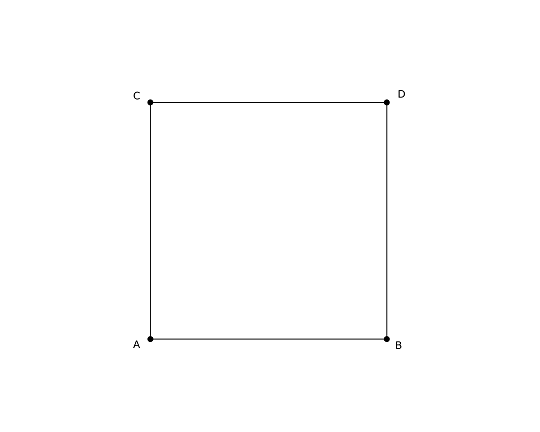
\includegraphics[width=0.5\textwidth]{figure5.png}
\caption{Square ABCD.}
\end{figure}

\begin{figure}
\centering
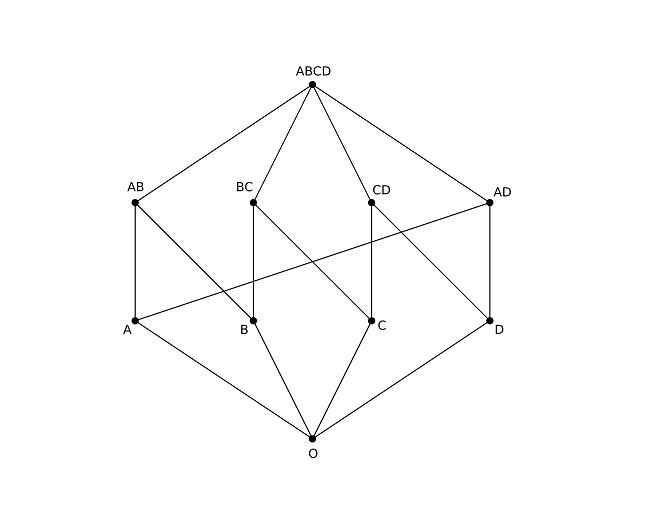
\includegraphics[width=0.5\textwidth]{figure6.png}
\caption{Its face lattice.}
\end{figure}


If anybody wants to read about this, then read ''Lectures on
Polytopes'' by Ziegler.

This can be applied to cubes, for example, as follows:

\begin{center}
  $(1 0 0 0 1 1)\left( \begin{array}{c} x_{1} \\ x_{2} \\ x_{3} \\
      x_{4} \\ x_{5} \\ x_{6} \end{array} \right) \leqslant k$,
\end{center}

where $k$ represents the non-zero entries (in this case $k = 3$), and
using this, we can calculate the barycenters.


% Local Variables: 
% mode: latex
% TeX-master: "dag-2011"
% End: 
 